\section{Prototypes}
This section will describe the setup of the prototypes developed during this project.
\todo[author=Thalley]{When the section is more done, improve the introduction}

\subsection{Prototype \#1}
\label{sec:implementation:prototypes:prototype1}
The first prototype was an Android phone application, 
that showed the location of the user, 
the direction the phone was pointing, 
and the devices that were being pointed at.
The application used a $10 \times 10$ grid to simulate a square room, 
in which the user and the devices to be controlled were located.
A set of imaginary devices was hardcoded into the application with fixed positions, 
and the grid would look like the one shown in \Cref{table/prototype-grid}.
The user is positioned in the center at $(5,5)$ by default. 
This position can be changed by using the \texttt{Up}, \texttt{Down}, \texttt{Left} and \texttt{Right} buttons.
When the user's direction changes, 
a list of devices being pointed at is acquired, 
by calculating the angle between the user's position and the position of each device.
The direction is found using magnetic fields, 
such that \num{0} is north, \num{-90} is west, \num{90} is east, etc. 
The angle between each smart device and the user, 
is calculated finding the inverse tangent (arctangent), 
and then converting from radians to degrees (dividing \num{180} by $\pi$), 
such that we get:
\begin{equation}\label{eq:angle}
\var{angle} = 180 / \pi * \arctan(\var{user.y} - \var{device.y} / \var{user.x} - \var{device.x})
\end{equation}
where \var{user.x} and \var{user.y} are the $x$ and $y$ coordinates of the user and likewise for the device.
A screenshot of this application is shown in \Cref{fig:prototype1-app-screenshots}.

% Thalley: Måske lave om et et Tikz coordinatsystem i stedet for? Fylder unødvendigt meget imo. 
\begin{table}[!htb] 
    \centering
    \tiny
    \begin{TAB}(e){|c:c:c:c:c:c:c:c:c:c|}{|c:c:c:c:c:c:c:c:c:c|}
     &  &  &  &  &  &  &  &  & Stereo \\
     &  &  &  &  &  &  &  &  &  \\
     &  &  &  &  &  & \begin{tabular}[c]{@{}l@{}}Coffee\\ Maker\end{tabular} &  &  &  \\ 
     &  &  &  &  &  &  &  &  &  \\ 
    \begin{tabular}[c]{@{}l@{}}Garage\\ Door\end{tabular} &  &  &  &  &  &  &  &  &  \\ 
     &  & Lamp 2 &  &  &  &  &  &  &  \\
     &  &  &  &  &  &  &  &  &  \\ 
     &  &  &  &  &  &  &  &  &  \\ 
     &  &  &  &  &  &  &  &  &  \\ 
    Lamp 1 &  &  &  &  & TV &  &  &  &  \\
    \end{TAB}    
    \caption{Grid showing the position of devices. Lamp 1 is located at (0,0) and Stereo is located at (9,9)}
    \label{table/prototype-grid}
\end{table}

\begin{figure}[!htb]%
    \centering
    \subfloat{
        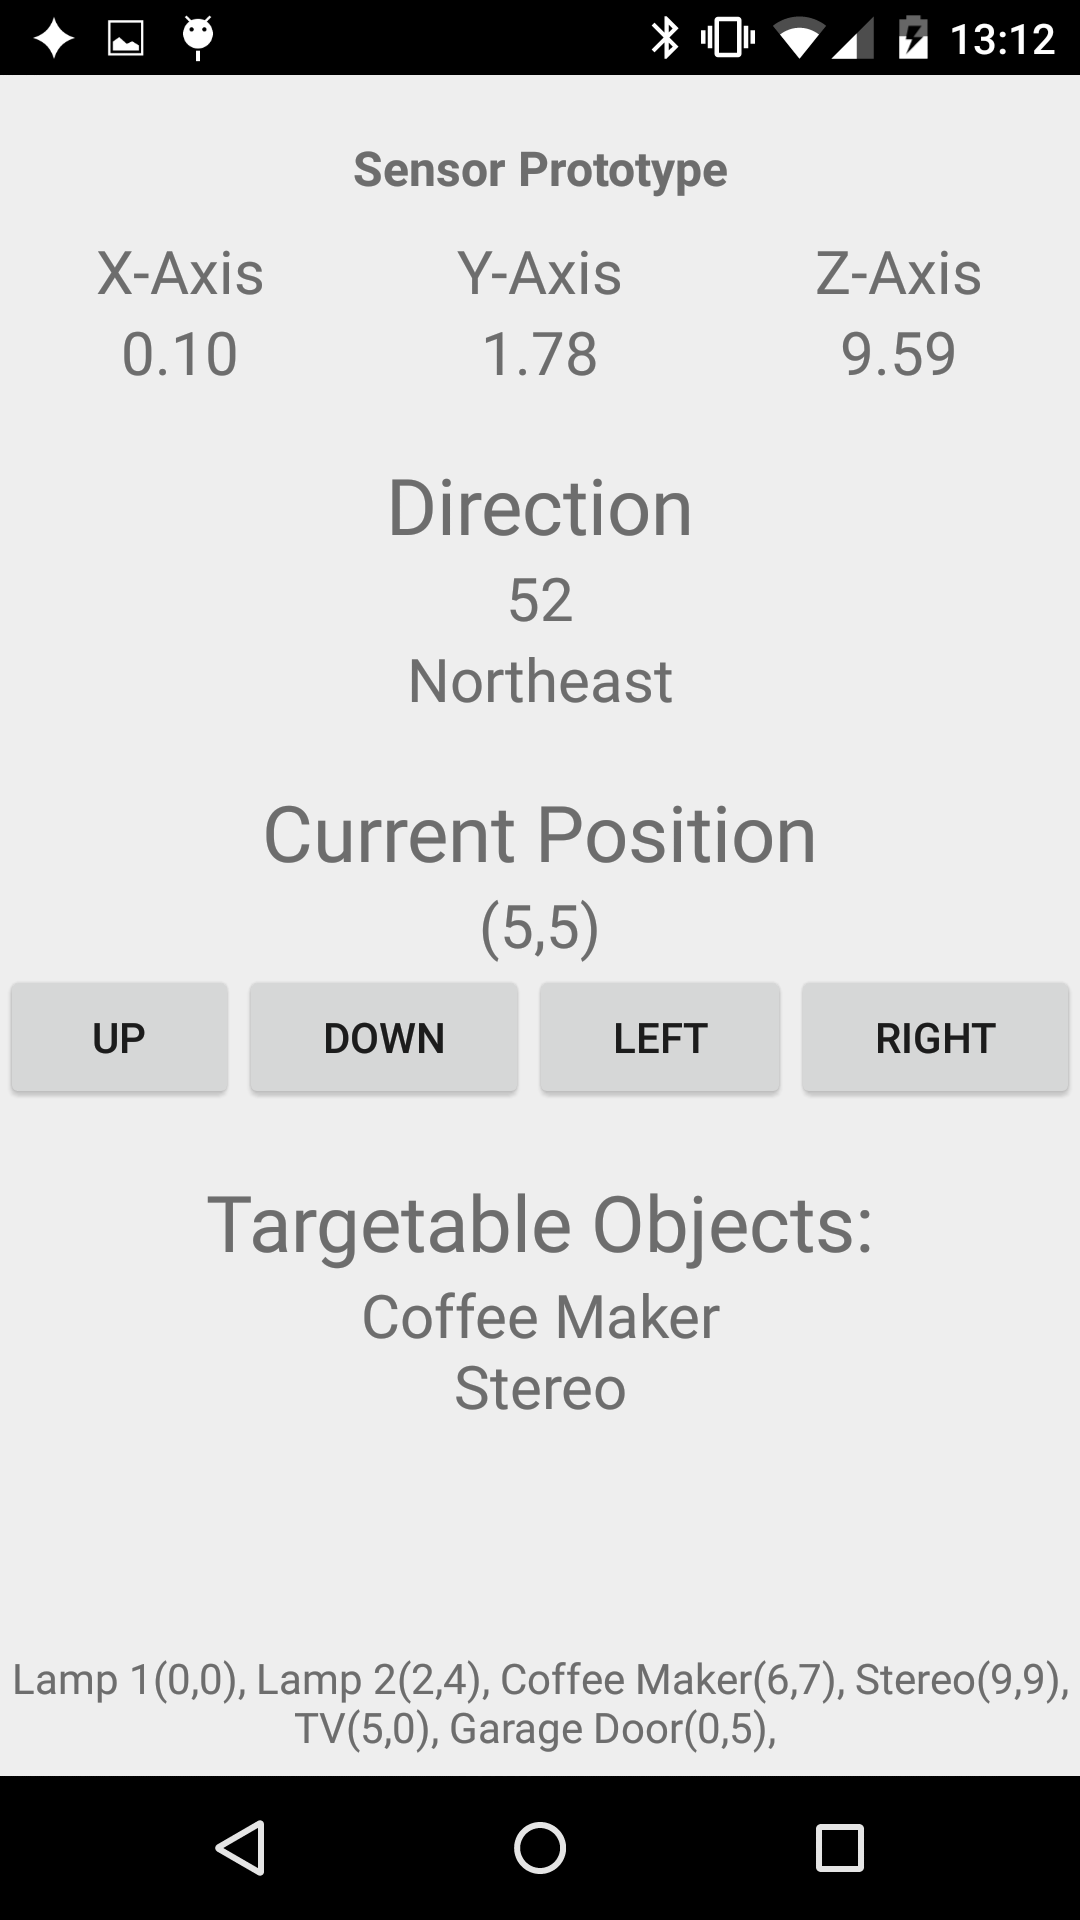
\includegraphics[width=0.3\textwidth]{images/Prototype1_Android_1.png}
    }
    \subfloat{
        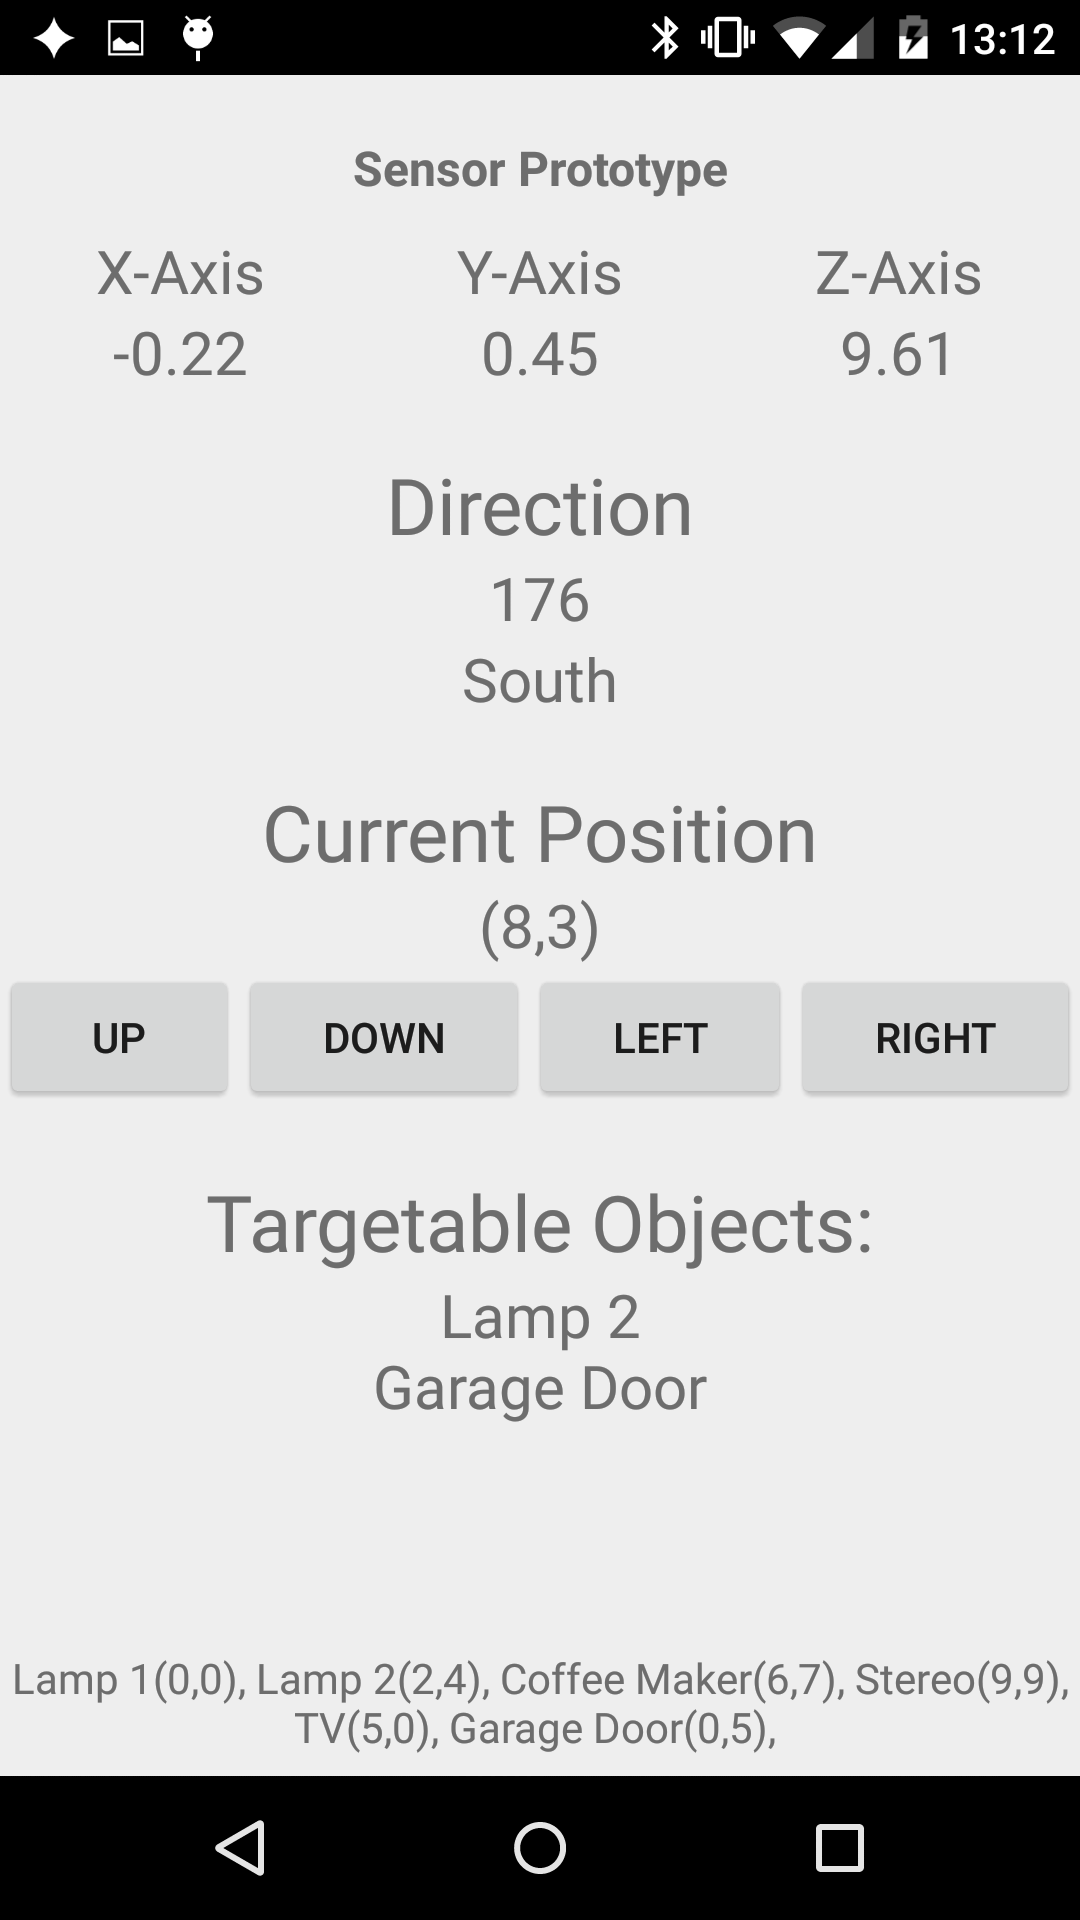
\includegraphics[width=0.3\textwidth]{images/Prototype1_Android_2.png}
    }
    \caption{Screenshots of the first prototype.}
    \label{fig:prototype1-app-screenshots}
\end{figure}

\FloatBarrier
\subsection{Prototype \#2}
\label{sec:implementation:prototypes:prototype2}

The second prototype consisted of an iOS application, 
similar to the Android application described in section \ref{sec:implementation:prototypes:prototype1}, 
and a server that represented two controllable lamps.
The platform was changed from Android to iOS, 
because Estimote does not have a SDK for Android.

\subsubsection{Major Changes}
\begin{itemize}
    \item Introduction of a server for the application to interact with.
    \item Switched platform from Android to iOS.
\end{itemize}

In this prototype the room is still represented as a grid, 
and the user is placed in the center of the grid, 
however the user is unable to change position.
This is because the first prototype showcased the idea of pointing at devices from different locations sufficiently, 
and the next step would be to use the actual location of a user using Estimote beacons.
As shown in \Cref{fig:prototype2-app-screenshots}, 
the user can see his direction as an angle between himself and north.
The angle is computed the same way as in Prototype 1 with \Cref{eq:angle}.

Devices are represented as orange dots, 
and if the user points towards one of them, 
two buttons will appear that allow the user to interact with the device, 
by either turning it \texttt{on} or \texttt{off}.
When the user turns a device on or off, 
it will be reflected on the server, 
where a corresponding box will have the color \texttt{green} when turned on, 
and \texttt{red} when turned off as shown in \Cref{fig:prototype2-server-screenshot}.
The server is running as a Heruko\footnote{\url{https://heroku.com/}} application, 
as a simple RESTful webservice written in Python. 
The server contains the information of the devices, 
such as ID, name, status and position.
The application gets this information by sending a GET request, 
to get a list of all the devices and their information. 
To change the status of a device (turn off or on), 
the application sends a POST request with the device's ID and the action. 
In this prototype, the only actions are \texttt{turnOn} and \texttt{turnOff}.

\begin{figure}[!htb]%
    \centering
    \subfloat{
        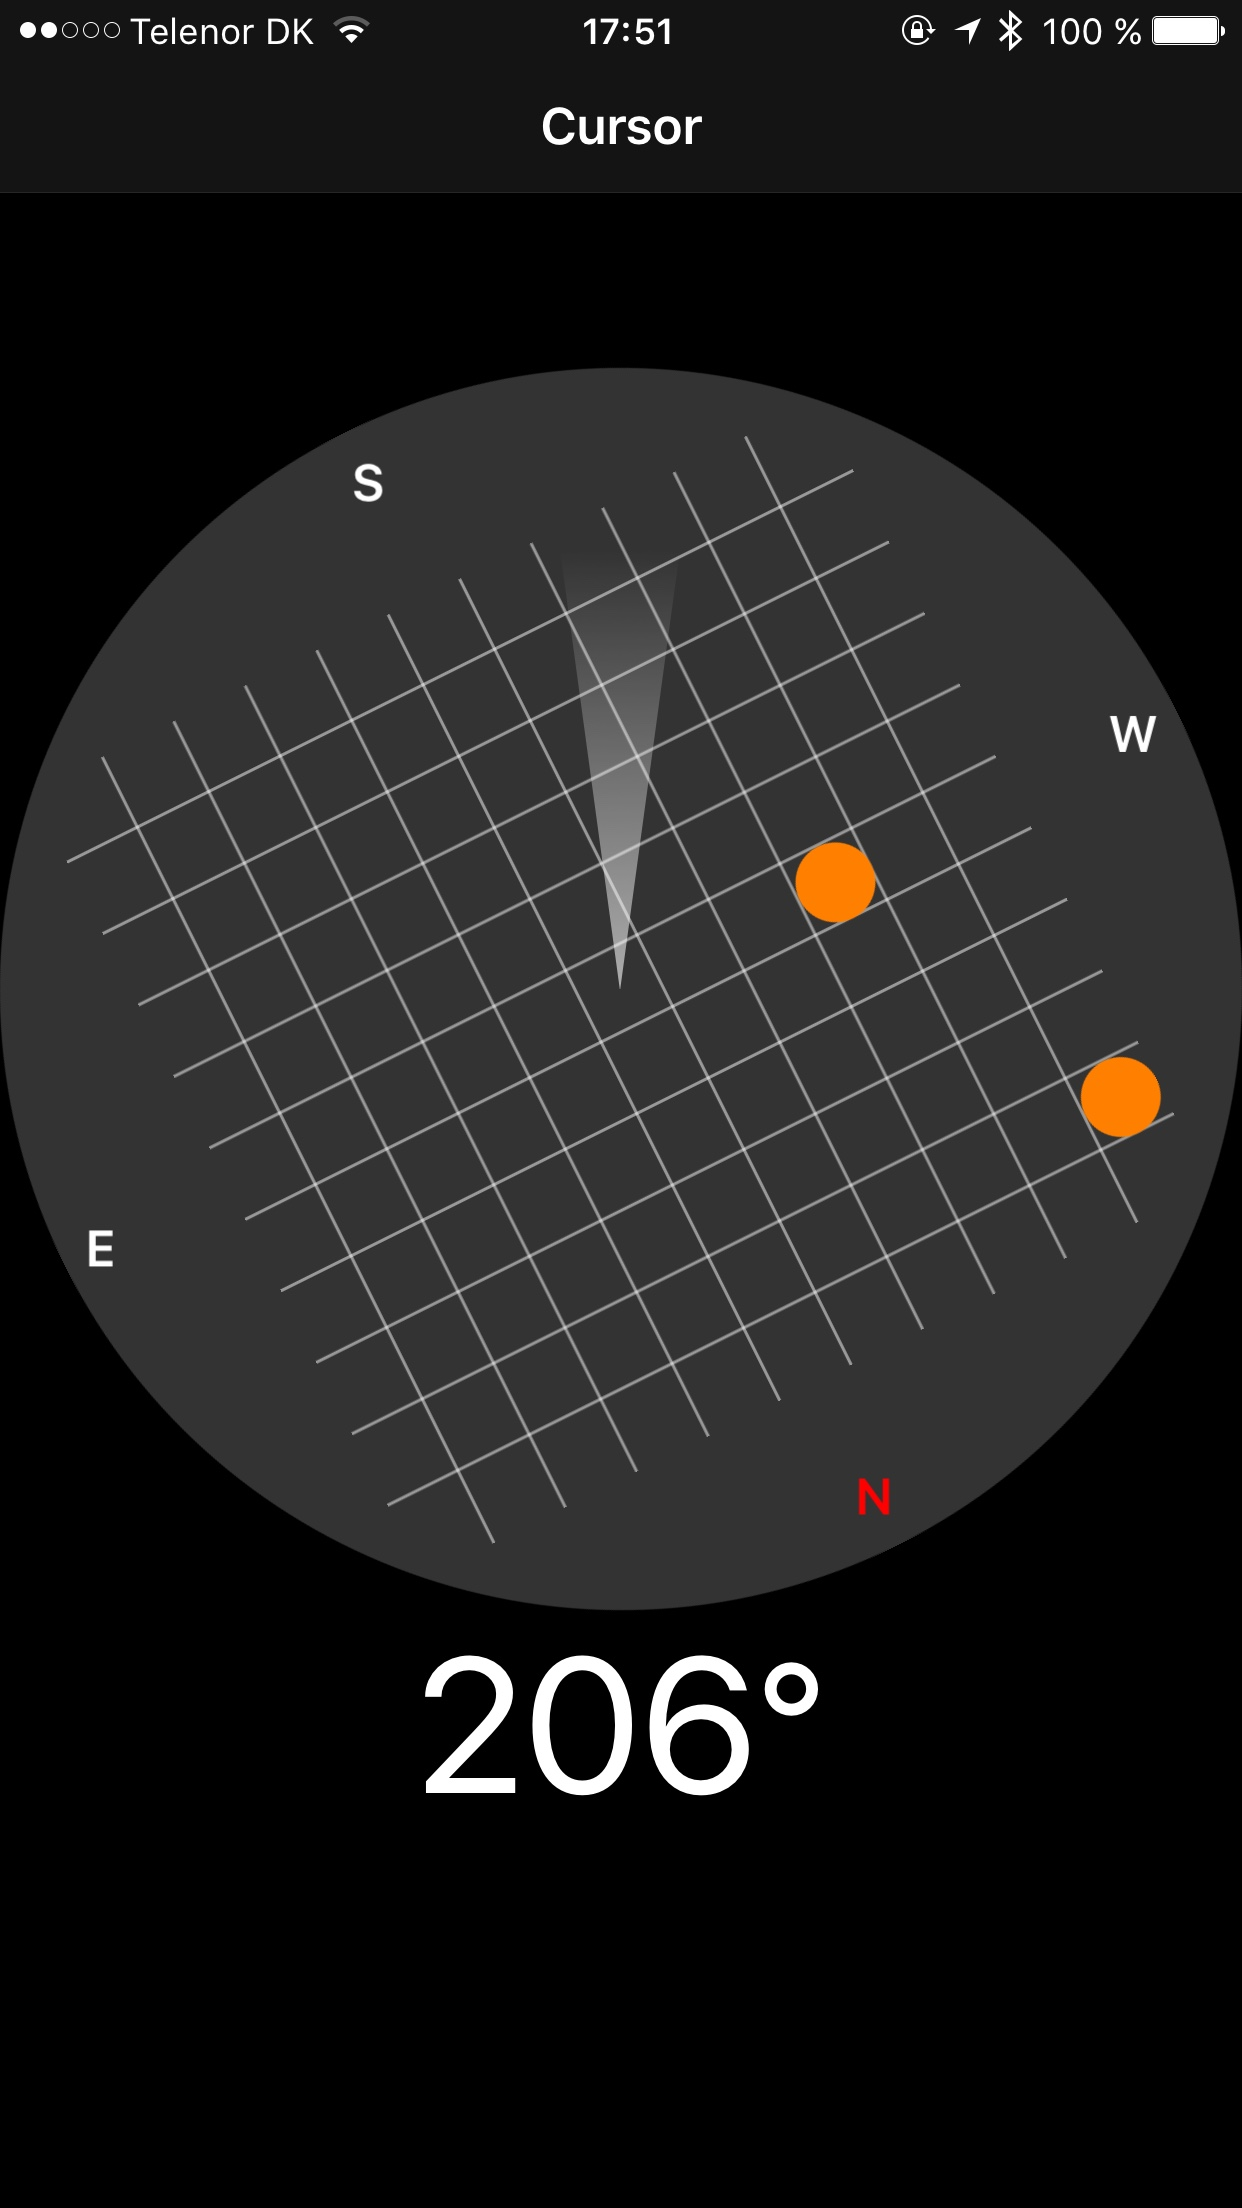
\includegraphics[width=0.3\textwidth]{images/Prototype2_iOS_1.png}
    }
    \subfloat{
        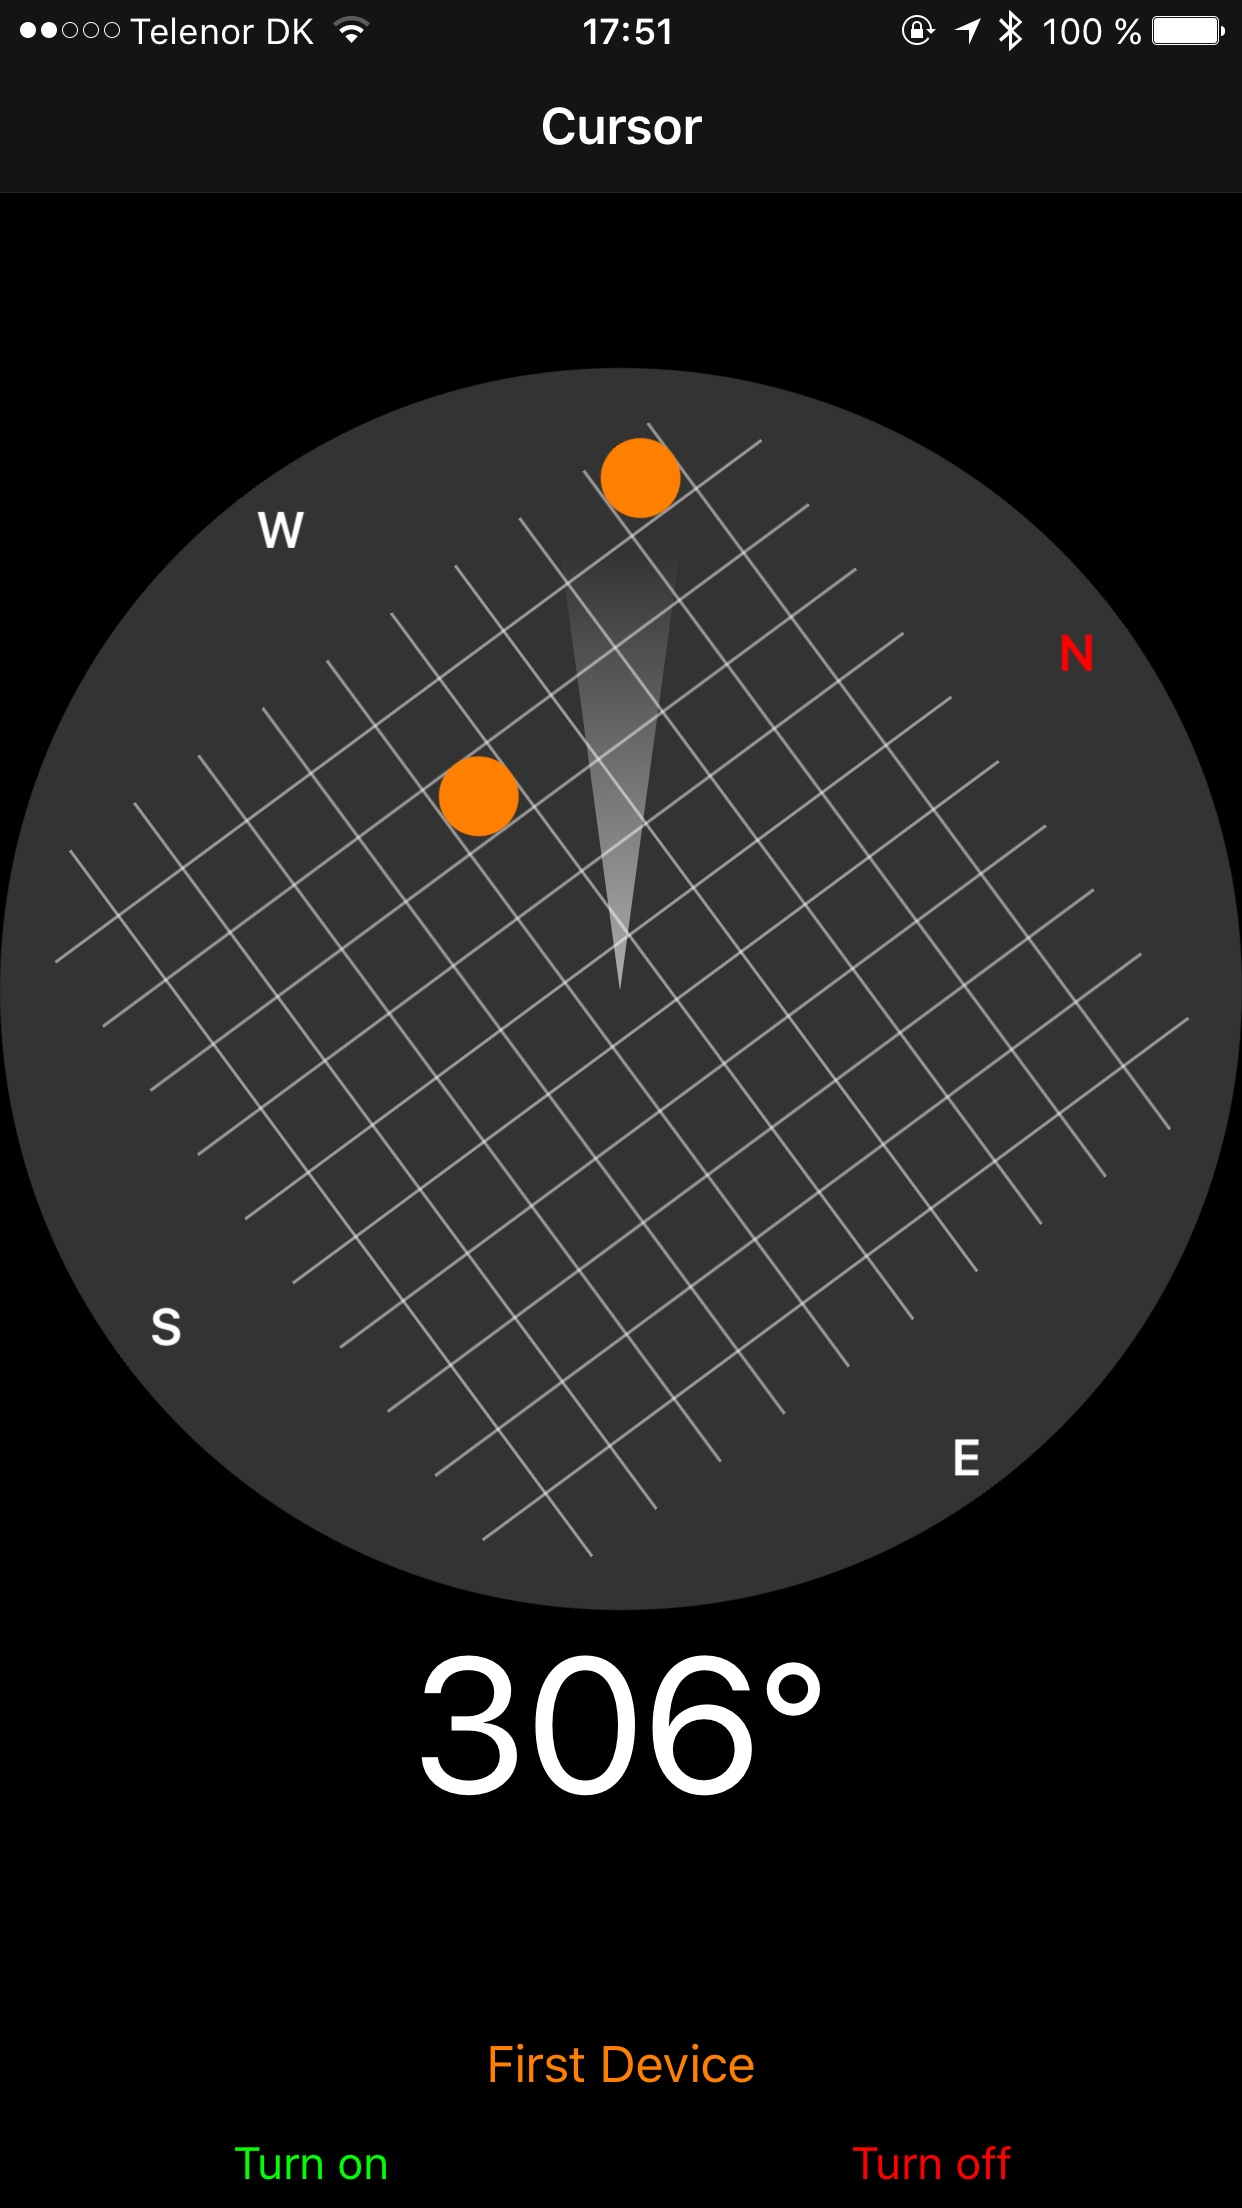
\includegraphics[width=0.3\textwidth]{images/Prototype2_iOS_2.png}
    }
    \caption{Screenshots of the second prototype application.}
    \label{fig:prototype2-app-screenshots}
\end{figure}

\begin{figure}[!htb]
    \centering
    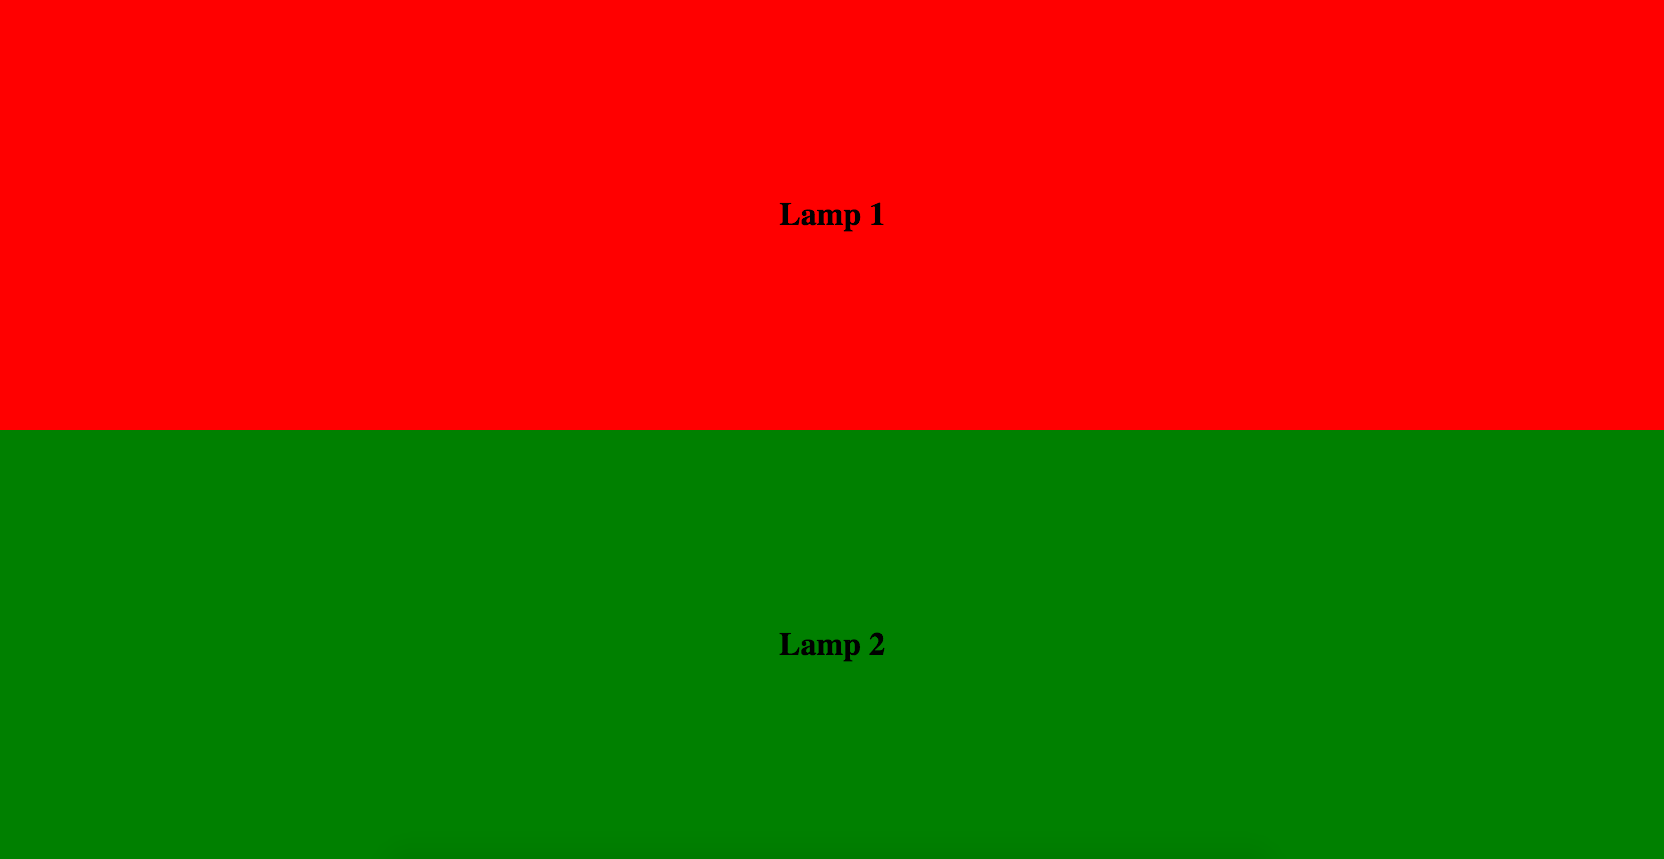
\includegraphics[scale=0.2]{images/Prototype2_Server.png}
    \caption{Screenshot of the server representing two lamps in the second prototype. Colors indicate their status. \texttt{Red} (top): Off and \texttt{Green} (bottom): On}
    \label{fig:prototype2-server-screenshot}
\end{figure}

\FloatBarrier
\subsection{Prototype \#3}
\label{sec:implementation:prototypes:prototype3}

The third prototype builds upon the second prototype for iOS, 
which was expanded to include some new features. 
The second prototype would assume that the user was positioned in the center of the room, 
but the new prototype takes the users position into account when determining devices being pointed at. 
Estimote beacons and the SDK provided by Estimote for indoor positioning was utilized, 
in order to determine the position of the user.

The indoor SDK from Estimote provides a visualization of the room, 
in which the positioning takes place, 
as well as a visualization of the installed beacons, 
and the position of the user. 
The view can be used to visualize custom objects. 
\Cref{fig:prototype3-room-screenshot} shows two red circles in the room. 
Each of the circles represent one of the virtual lamps introduced in the second prototype. 
The color of the lamp indicates the state the lamp is in. 
A lamp can either be on or off. 
The states are represented by red and green respectively.

Furthermore the prototype added support for training and recognizing gestures, 
using the \$3 Gesture Recognizer library described in \Cref{sec:threedollar}.
Users can add a gesture by giving the gesture a name, 
and train it at least five times. 
When added, the gesture can be used when pointing at a lamp, 
to toggle the state of the lamp. 
For example, if the user has trained a circle named ``Half Circle'', 
he can visit the screen showing his lamps and his position, 
point at one or more lamps and perform the ``Half Circle'' gesture, 
in order to either turn on or turn off the lamps.

The third prototype does not support associating a gesture with an action, 
\ie performing a specific action for a specific gesture. 
Nor does it support creating a model of a room. 
The prototype is limited to a specific room, 
modeled after the living room of one of the research members.

\subsubsection{Major Changes}
\begin{itemize}
\item Uses BLE beacons to position the user in a room, and take his position into account when determining devices being pointed at.
\item Adds training and recognition of gestures, in order to trigger actions of a controllable device.
\item Adds a graphical representation of the room, in which the beacons and the devices are installed.
\end{itemize}

\begin{figure}[!htb]%
    \centering
    \subfloat{
        \frame{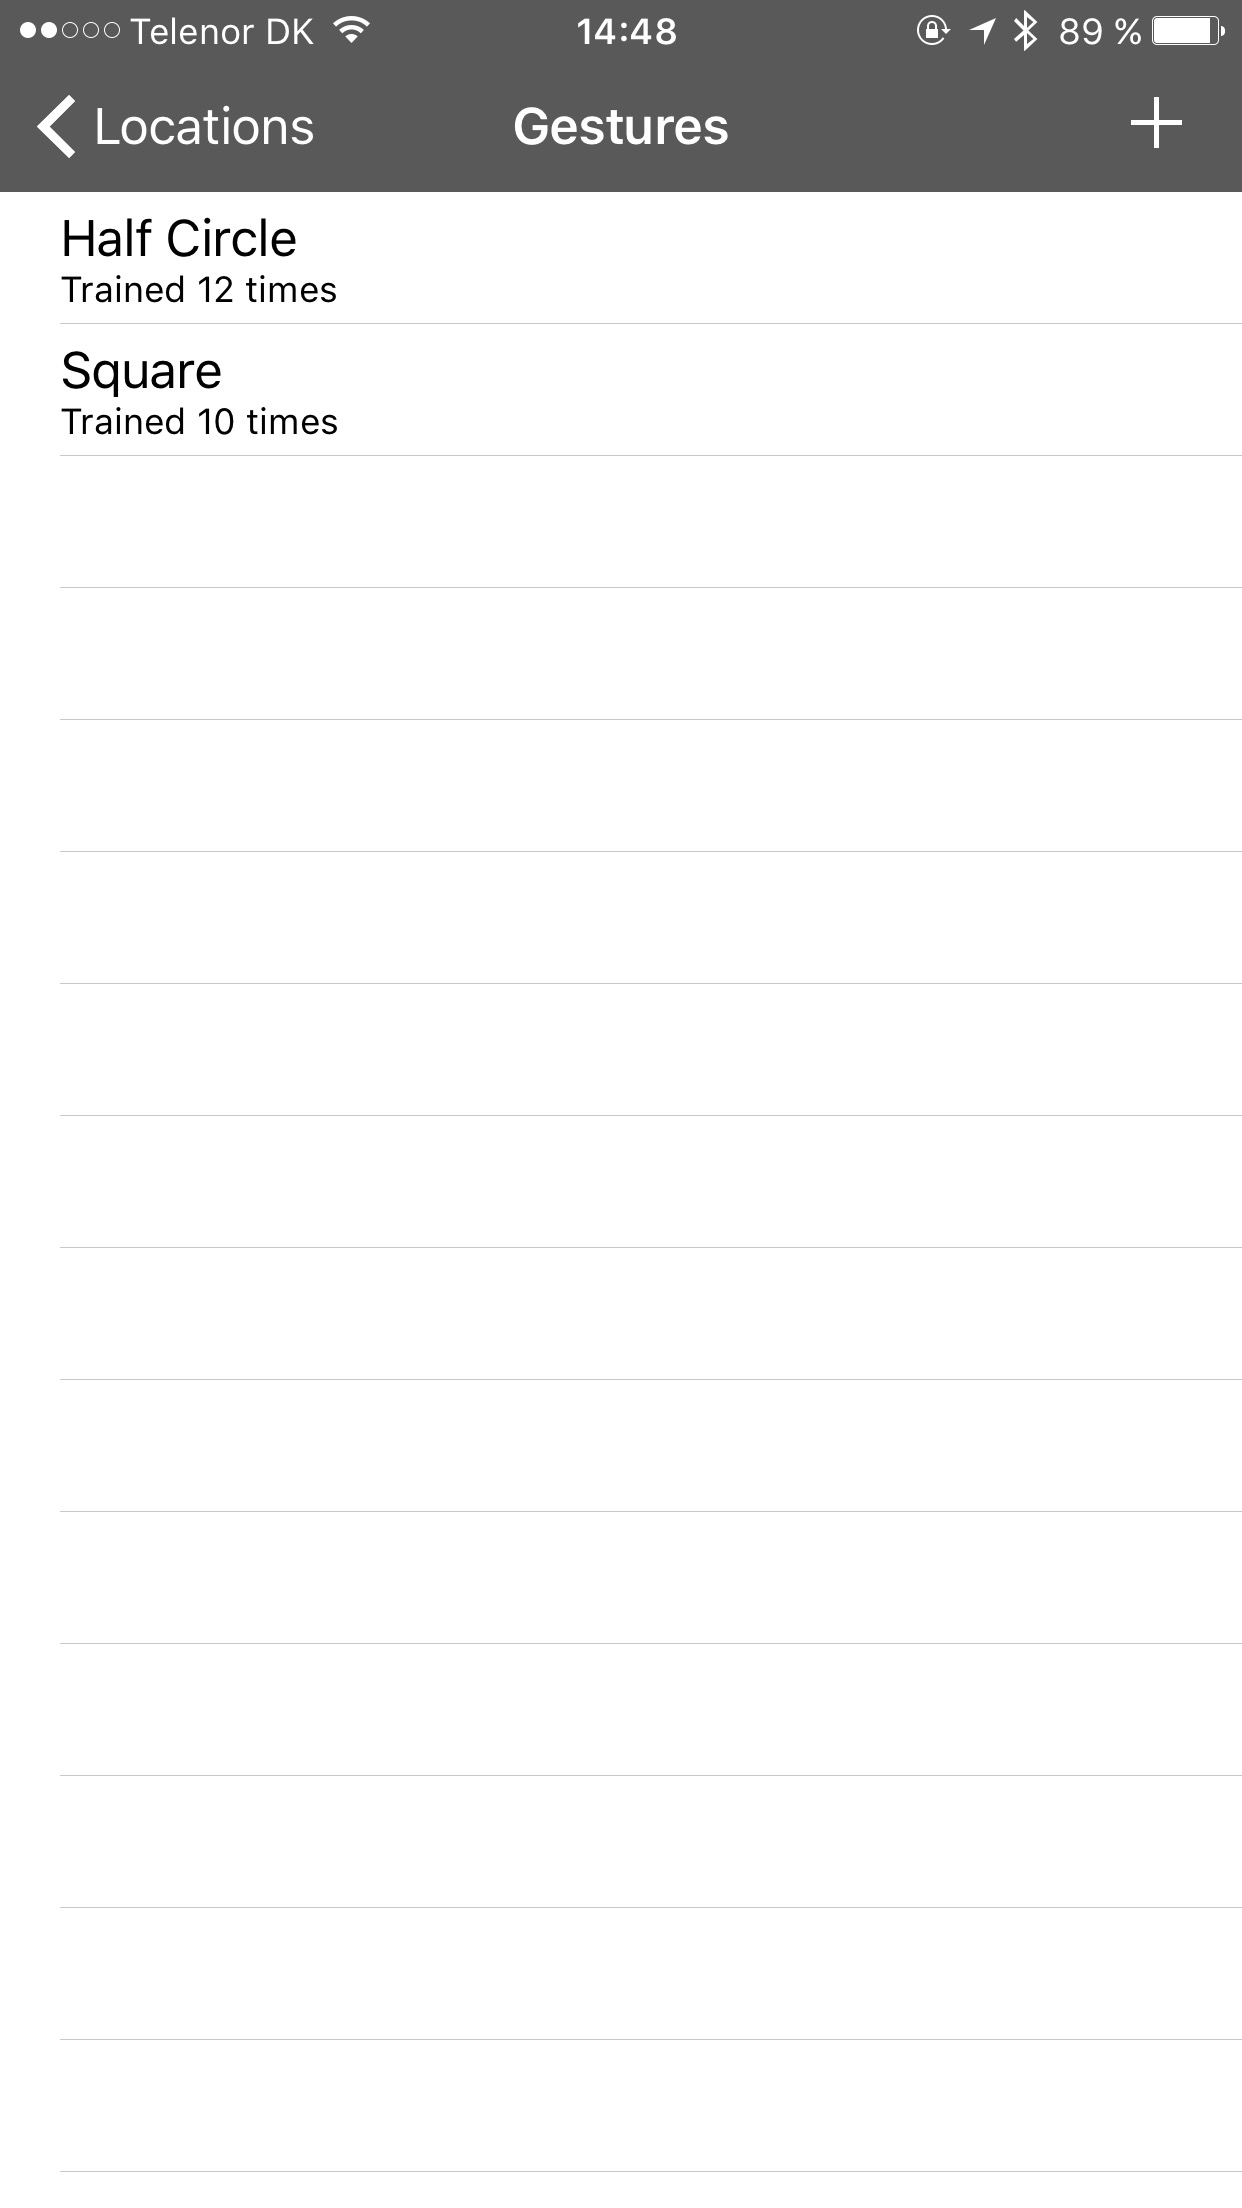
\includegraphics[width=0.3\textwidth]{images/prototype-3-all-gestures}}
    }
    \subfloat{
        \frame{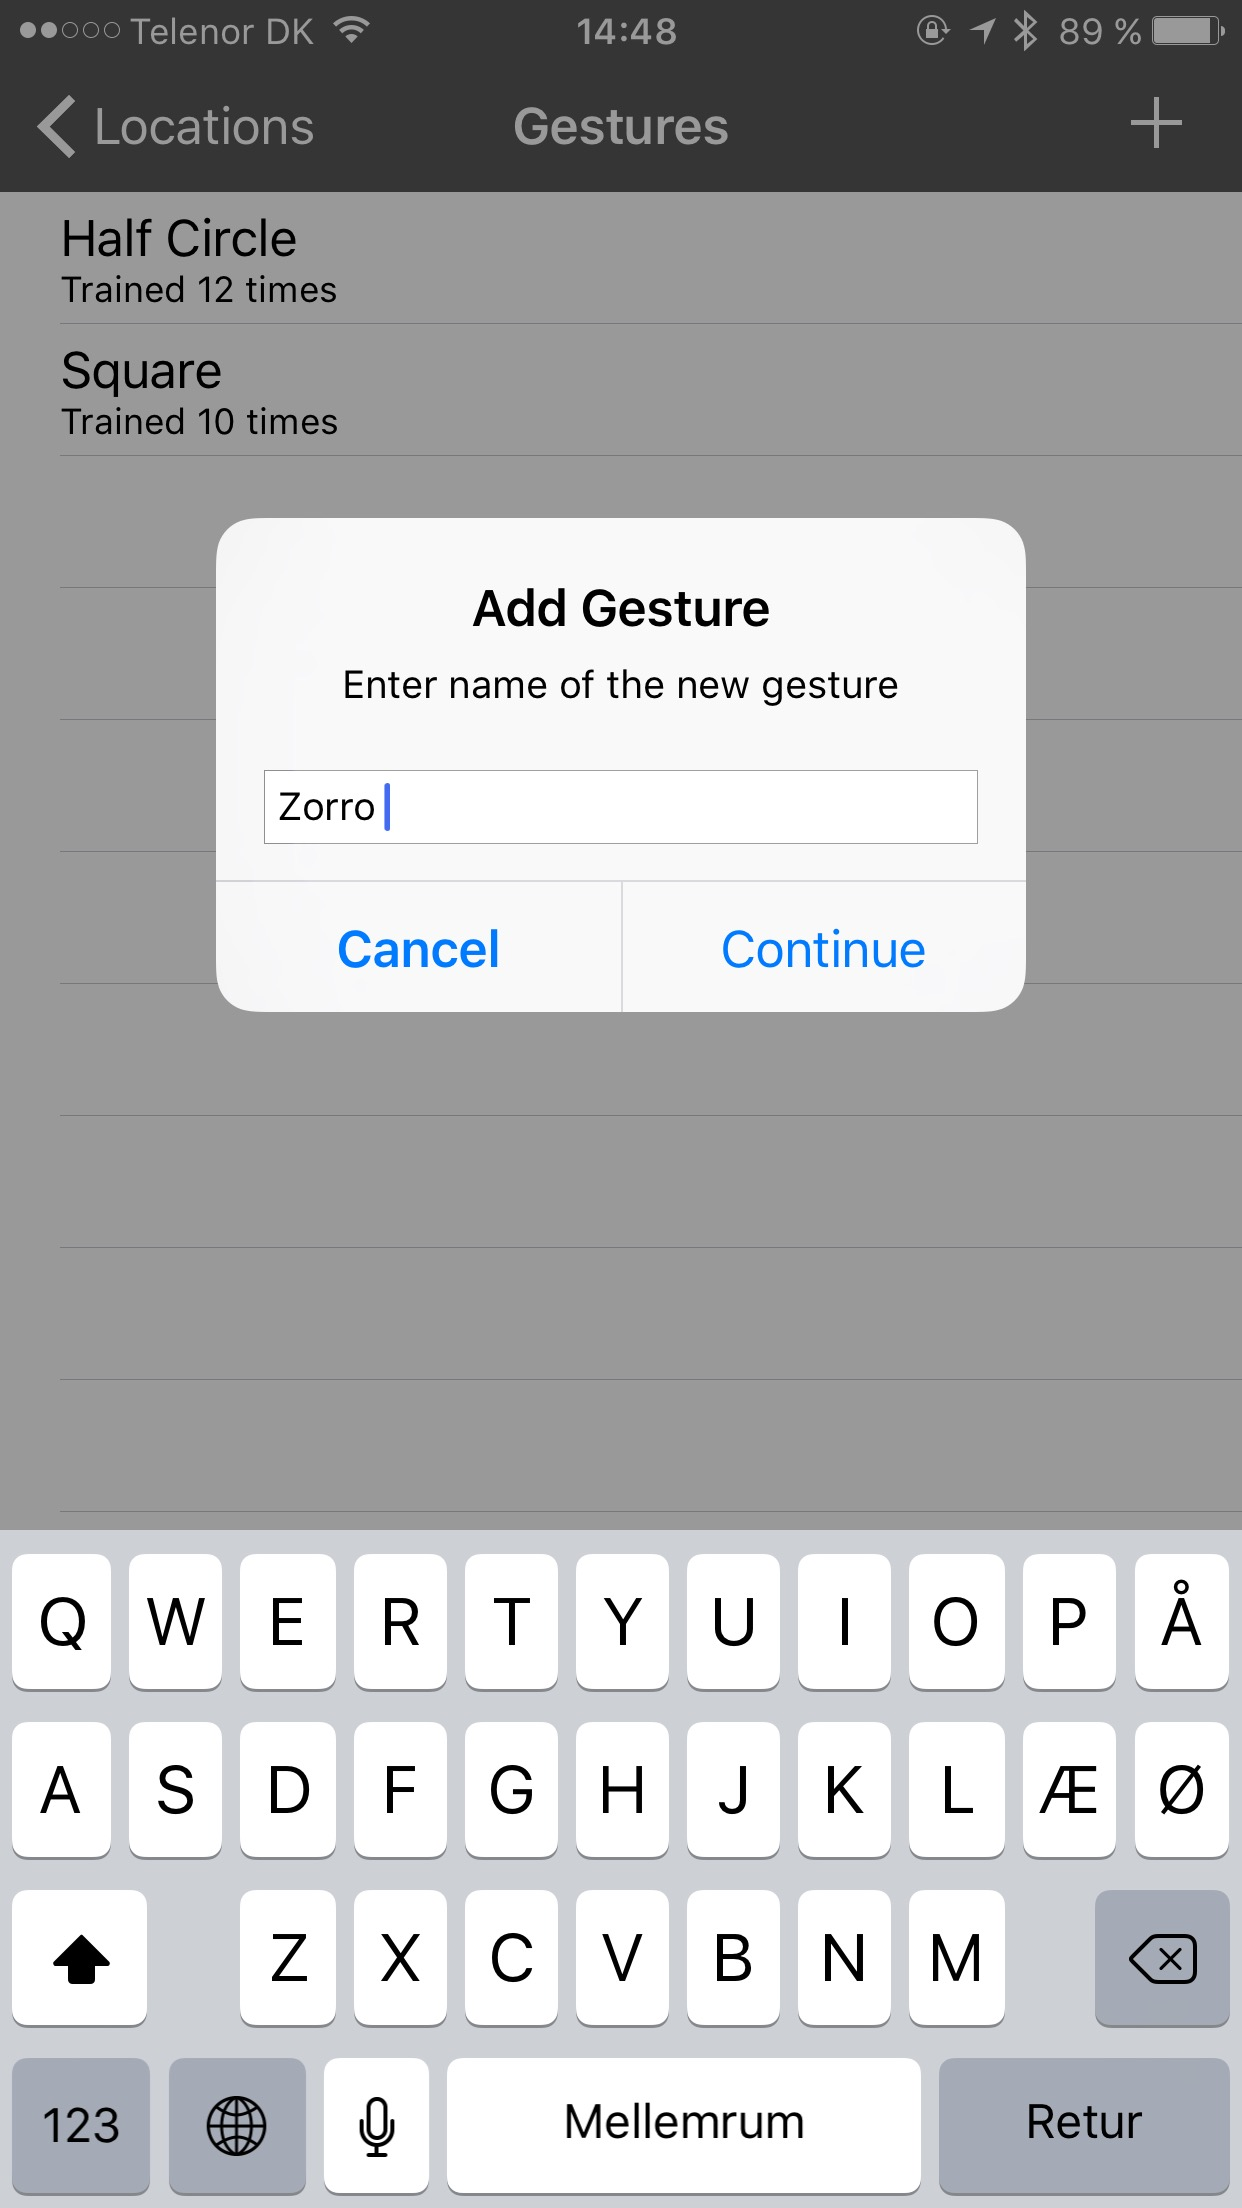
\includegraphics[width=0.3\textwidth]{images/prototype-3-new-gesture}}
    }
    \subfloat{
        \frame{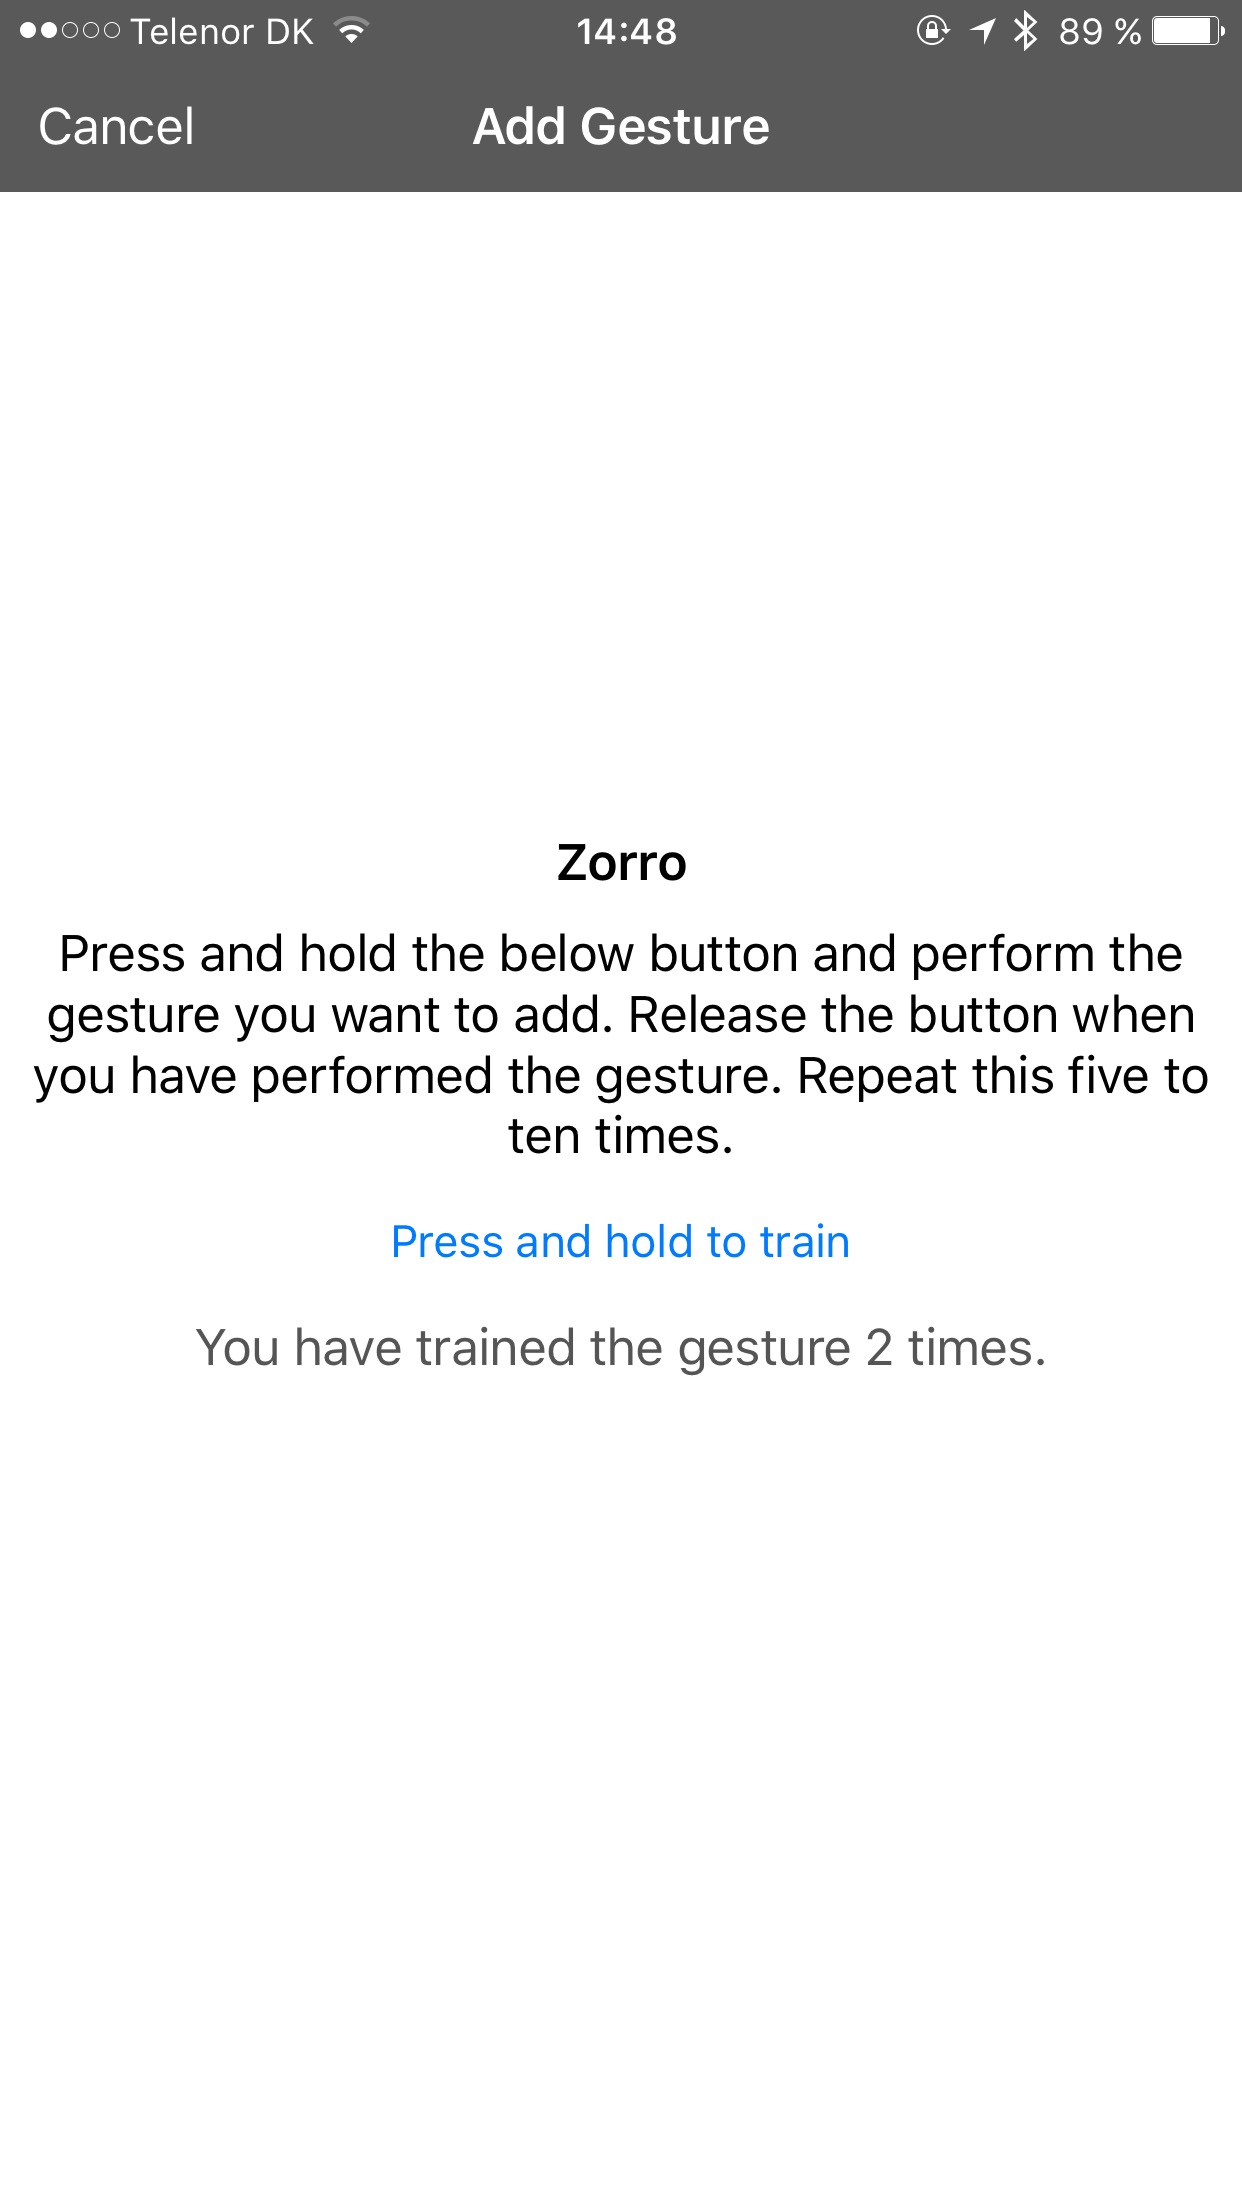
\includegraphics[width=0.3\textwidth]{images/prototype-3-train-gesture}}
    }
    \caption{Screenshots showing the flow and interface for adding and training a new gesture in the third prototype.}
    \label{fig:prototype3-gesture-screenshots}
\end{figure}

\begin{figure}[!htb]%
    \centering
    \frame{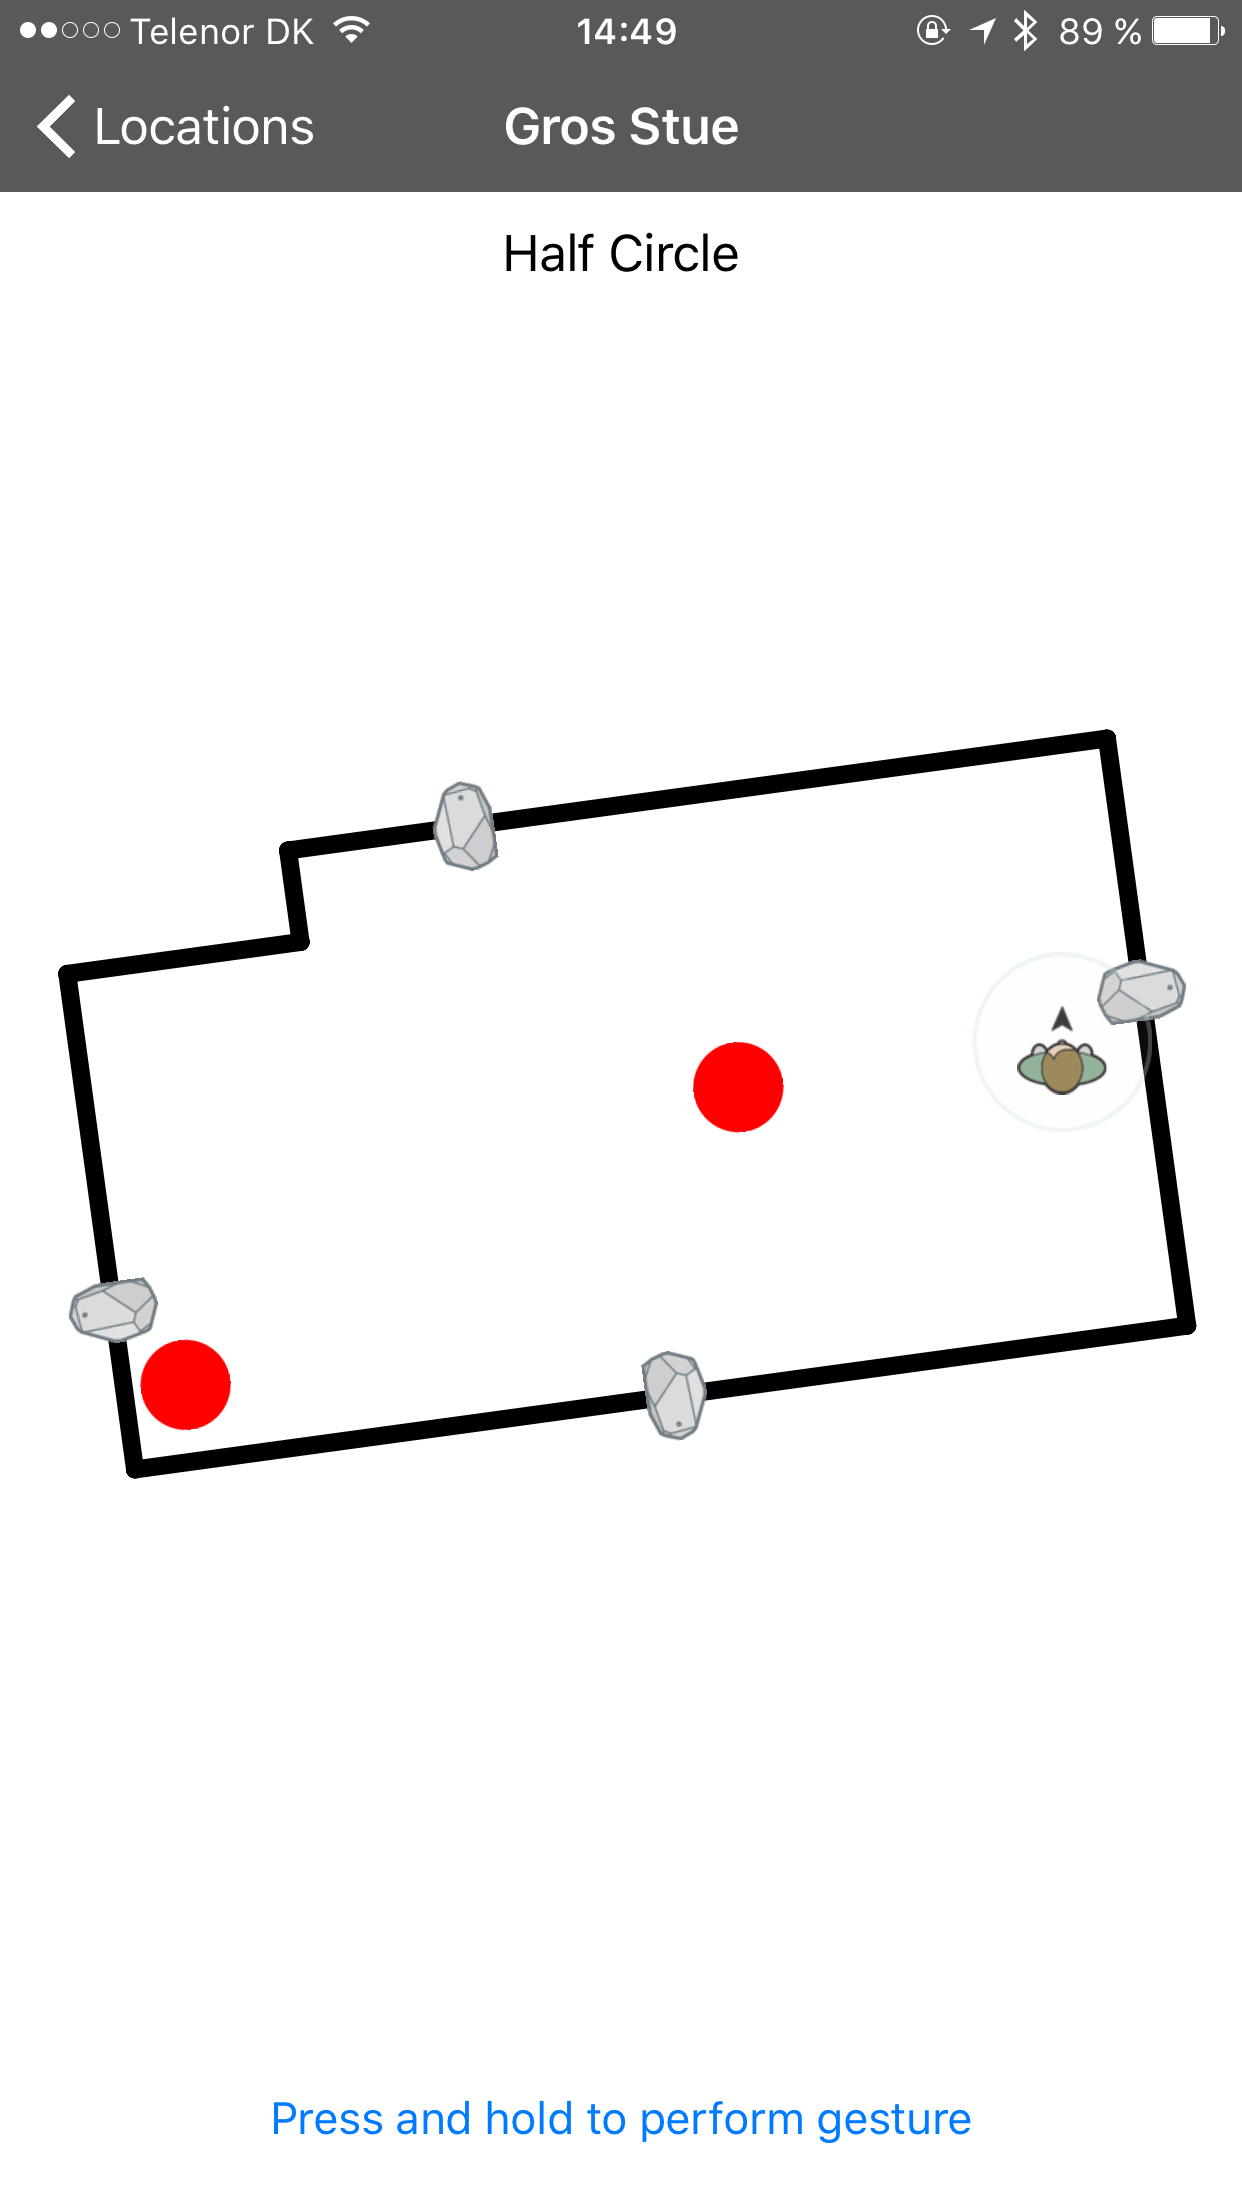
\includegraphics[width=0.3\textwidth]{images/prototype-3-gesture-triggered}}
    \caption{Screenshot showing new representation of the room and controllable devices. In this screenshot the gesture named ``Half Circle'' was recently recognized, and therefore the gesture name is shown in the top of the screen.}
    \label{fig:prototype3-room-screenshot}
\end{figure}

%%% Local Variables:
%%% mode: latex
%%% TeX-master: "../../master"
%%% End:
